\section{Energiekalibrierung des Spektrometers}
\subsection{Theoretische Grundlagen}
Die Energiekalibrierung eines Gammaspektrometers basiert auf der Zuordnung von Kanalnummern eines Multikanalanalysators (MCA) zu bekannten $\gamma$-Übergangsenergien. Hierfür werden Proben mit bekannten Zerfallsprofilen und spektraler Vielfalt verwendet. Der $^{152}$Eu-Kern eignet sich besonders gut für die Kalibrierung im Energiebereich zwischen etwa 100 keV und 1,4 MeV, da er eine große Anzahl von Gamma-Übergängen enthält. Zusätzlich wird der 662-keV-Übergang von $^{137}$Cs verwendet, um die Kalibrierung im mittleren Energiebereich zu stabilisieren.
\paragraph{$\gamma$-Spektrum von $^{152}$Eu}
Der Zerfall von $^{152}$Eu führt über mehrere angeregte Zustände des $^{152}$Sm zu einer Vielzahl charakteristischer $\gamma$-Linien.
%tabelle mit Energien und Intensitäten der Linien einfügen
Diese Linien dienen als Referenzpunkte für die Kalibrierung des Spektrometers.
Aufgrund der begrenzten Energieauflösung des Detektors können sich mehrere nahe beieinander liegende Übergänge überlappen und einen einzigen Peak bilden. Diese Überlappung tritt besonders häufig bei Spannungen unter 300 keV auf, da der Linienabstand dann kleiner als die Halbwertsbreite (FWHM) des Detektors ist.
Zur genauen Identifizierung der Linien wird eine Hintergrundmessung ohne Probe durchgeführt und anschließend vom Spektrum subtrahiert, um die Auswirkungen von Umgebungsstrahlung und elektrischem Rauschen zu eliminieren.
\paragraph{Lineare Energiekalibrierung}
Die Beziehung zwischen der Kanalnummer $K$ und der Energie $E$ eines $\gamma$-Übergangs wird durch eine lineare Funktion beschrieben:
\begin{align*}    
    E(K) = aK + b
\end{align*}
Die Parameter $a$ und $b$ werden durch eine lineare Regression der bekannten Energien der $^{152}$Eu-Übergänge gegen die gemessenen Kanalnummer bestimmt. \\
Dazu wird noch der $^{137}$Cs-Peak verwendet, um die Kalibrierung im mittleren Energiebereich zu stabilisieren und systematische Unsicherheiten zu reduzieren.
\paragraph{Detektoreffizienz}
Die Wahrscheinlichkeit, dass ein $\gamma$-Photon mit der Energie $E$ im Detektor ein vollständiges Signal erzeugt, wird mit der Detektoreffizienz $\epsilon(E)$ beschrieben. Diese hängt von der gemessenen Peakfläche $A(E)$, der Anzahl der emittierten $\gamma$-Photonen $N_\gamma(E)$ und der Messzeit $t$ ab:
\begin{align*}  \epsilon(E) = \frac{A(E)}{N_\gamma(E) \cdot t}  \end{align*}
Die absolute Aktivität der Probe ist unbekannt, also kann nur die relative Effizienz bestimmt werden. Aber das ist für die Energieabhängigkeit der Effizienz ausreichend, denn der unbekannte Proportionalitätsfaktor ist für alle Energien der gleiche und fällt beim Normalisieren während der Analyse weg.\\
Im üblichen Fall fällt die Detektoreffizienz mit steigender Energie ab, denn hochenergetische $\gamma$-Photonen haben eine geringere Wahrscheinlichkeit, vollständig im Detektor absorbiert zu werden. (Daher ist es wichtig, die Effizienzkurve über den gesamten Energiebereich zu bestimmen, um die gemessenen Spektren korrekt interpretieren zu können.)
\subsection{Durchführung}
Zunächst wird der Detektor in einem Winkel von 90° ausgerichtet, sodass er direkt auf die Probenhalterung zeigt. Während dieses Vorgangs bleibt die Cäsiums-Quelle geschlossen; die Europiumkomponente mit geringer Aktivität wird an die Targethalterung angebracht. Mit dieser Versuchsanordnung soll der Einfluss der Hintergrundstrahlung der Cäsium-Quelle auf die Messung minimieren werden.

Die Messungen wurden mit einer Totzeit von 300 s durchgeführt (mit als auch ohne die Europiumquelle). Das resultierende Hintergrundspektrum wurde dazu verwendet, den dem Cäsium zuzuschreibenden Hintergrund zu eliminieren.
\subsection{Auswertung}
Die gemessenen Spektren werden mittels eines Peak-Fitting-Algorithmus gefittet, um die den Peaks entsprechenden Kanalnummern zu ermitteln. Anschließend werden die bekannten Intensitäten der modifizierten $^{152}$Eu-Probe mit den gemessenen Kanalnummern verglichen, um die Kalibrierungsparameter $a$ und $b$ zu bestimmen. Die Energieeffizienz des Detektors wurde durch den Vergleich des gemessenen Bereichs mit dem Referenzwert evaluiert, wobei die Probeneigenschaften sowie die Messdauer berücksichtigt wurden. Die Ergebnisse werden in Form von Kalibrierungskurven und Effizienzgrafiken dargestellt, um die Robustheit des Detektors zu veranschaulichen.\\
\begin{figure}[htbp]
    \centering
    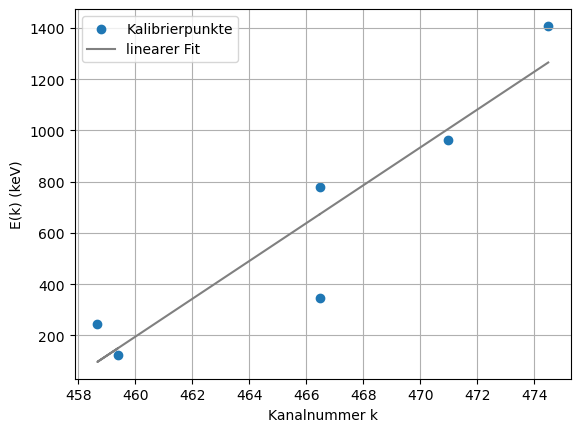
\includegraphics[width=0.75\textwidth]{figs/kalibrierung_1.png}
    \caption{Frontales Kalibrations-Spektrum der $^{152}$Eu-Quelle. Die Fehler wurden nicht dargestellt, da diese in der Darstellung zu dominant sind und nicht sinnvoll im Plot integriert werden können.}
    \label{plot:plot1}
\end{figure}
\FloatBarrier
Abbildung \ref{plot:plot1} zeigt mehrere Emissionslinien, von denen ??? eindeutig identifiziert werden können. Der Ursprung dieser Linien wird aus dem $^{152}$Eu-Zerfallchema \ref{} sowie aus den Summenpeaks und charakteristischen Röntgenanregungen der Quelle abgeleitet. Eine Analyse jeder einzelnen Komponente ist jedoch für die Abschätzung der Robustheit nicht erforderlich und würde den Rahmen der vorliegenden Studie sprengen.
\\
Auf der Grundlage der Anpassungsgleichung für die Kanalenergie (Gleichung \ref{}) und der vorgeschlagenen linearen Bereiche (siehe Anhang?, Tabelle \ref{}) wurden die den Kanälen entsprechenden Energien in keV ermittelt, wie in Abbildung 7 dargestellt. Die Anpassungsparameter für die verwendete lineare Gleichung (Gleichung \ref{}) lauten wie folgt:
\begin{align*}
    a = 73.84411\pm 14.51236 \text{ keV/Kanal} \\
    b = -33773.36 \pm 6764.37 \text{ keV}
\end{align*}

